\documentclass[11pt]{article}
\usepackage[margin=1in,includefoot]{geometry}
\usepackage{fancyhdr}
\pagestyle{fancy}
\usepackage{graphicx,wrapfig,lipsum}
\fancyfoot{}
\fancyfoot[R]{\thepage}
\usepackage{color}
\usepackage{amsmath}
\usepackage{graphicx}
\usepackage{gensymb}
\usepackage{subcaption}
\usepackage{float}
\usepackage{multicol}
\setlength{\columnsep}{1cm}
\usepackage{tabularx}
\usepackage{hyperref}
\usepackage{multirow}
\usepackage{textcomp}
\usepackage{mathrsfs,amsmath} 
\usepackage{pdfpages}
\usepackage{amssymb}
\usepackage{xcolor}
\usepackage[nottoc]{tocbibind}

\usepackage{fontspec}
\setmainfont{Times New Roman}


\begin{document}

\begin{titlepage}
\begin{center}
   \textsc{\large DEPARTMENT OF ELECTRONICS AND TELECOMMUNICATION ENGINEERING\\
   [2mm]
   UNIVERSITY OF MORATUWA}\\
   [0.75cm]
   \begin{figure}[H]
   \centering
   
\includegraphics[height=1.9in]{UoM.png}\\
   [1.5cm]
   \end{figure}
   
   \MakeUppercase{\textsc{\LARGE EN2090 - LABORATORY PRACTICE II}}\\
   [2mm] 
   \line(1,0){350}\\
   [1mm]
    \huge{\bfseries LINEAR POWER SUPPLY} \\
   \line(3,0){350}\\
[1.2cm]  
\end{center}
\begin{minipage}{0.5\textwidth}
\begin{flushleft}
    \textbf{\large Name}\\
    \text{\large Munasinghe B.S.V.W.  }\\
    \text{\large Munasinghe M.M.R.H. }\\
    \text{\large Nifla M.N.F.}\\
    \text{\large Nushath M.N.M.}\\
    
\end{flushleft}
\end{minipage}
\hfill
\begin{minipage}{0.5\textwidth}
\begin{flushright}
    \textbf{\large Index Number}\\
    \text{\large 190397E}\\
    \text{\large 190399L}\\
    \text{\large 190413D}\\
    \text{\large 190423H}\\
\end{flushright}
\end{minipage}\\
[1.2cm]
\begin{center}
This report is submitted as a partial fulfilment of the module EN2090 - Laboratory Practice II.\\
\line(10,0){50}\\
[0.5cm]
\today
\end{center}
\end{titlepage}

\tableofcontents
\newpage

\pagenumbering{arabic}

\begin{multicols}{2}
\section*{Abstract}
Power supplies that are available in the market can be either Linear power supplies or switch-mode power supplies. Both have their advantage and disadvantage. Our task in this project was to design a high power, constant voltage DC power supply for a given rating. \\
\section{Introduction}
The given task was to design a high power constant voltage dc power supply without using any digital electronic components or ICs. the power supply should provide constant 10V DC power to the load at a power rating of 100W and the design should withstand a maximum of 10A current.\\
Our design is a Linear Power Supply that is better than Switch Mode Power Supplies in terms of cost, simpler design, low noise, and performance. Although they do better in these, they are inefficient and produce more heat than Switch mode power supplies. Given the circumstances and the needs, we go with LPS.\\
Linear Power supplies consist of 4 major phases: Transformer,  rectification, filtering, and regulation. Further for the protection against high currents, there is a need for a protection circuit. \\
In order to decide appropriate methods of implementation, selection of components, modeling, and calculations we went on a literature review.
\subsection{Literature Review}
\subsubsection{AC step down}
Most of the power supplies get the input from ac supply. Therefore it is a must to have a step-down transformer. This also served to isolate the power supply from the mains input for safety. The primary and the secondary turns ratio will ultimately define the voltage secondary voltage that will be used for the rest of the power supply circuitry. Inductance, turns ratio and voltage ratios are related with the following equation,\\
$$\frac{V_p}{V_s} = \frac{N_p}{N_s} = \sqrt{\frac{L_p}{L_s}}$$
\subsubsection{Rectification}
Full-wave rectification of ac wave from the secondary windings of the transformers is required for higher rms of the voltage. Center tapped or bridge rectifier serves this purpose. The bridge rectifier is preferred over center-tapped rectifier due to the following reasons: no need for ground the output terminal, The transformer is less costly as it is required to provide only half the voltage of an equivalent center-tapped transformer used in a full-wave rectifier, The PIV is one half that of center-tap rectifier.\\
PIV ratings of the rectifier are a major concern in the implementation of the circuit. Required PIV ratings can be calculated from the following equation,\\
$$PIV = V_p(sec) - 0.7V$$
The output voltage that appears after rectifier can be calculated from,\\
$$V_p(out) = V_p(sec) - 1.4V$$
\subsubsection{Filtering}
Smoothing the rectified DC output is required to reduce the ripple which is another step towards a linear power supply.\\
Ripple voltage and the capacitance are related with the below equation,
$$V_{ripple} = \frac{I_{max}}{2fC}$$
The capacitor value can be determined according to the ripple we want and vise-versa.\\
\end{multicols}
\newpage
\begin{figure}[H]
   \centering
   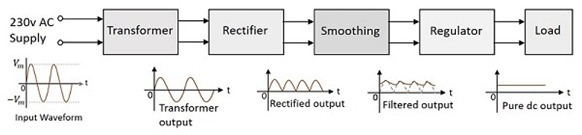
\includegraphics[height=1.2in]{Block_Diagram.jpeg}\\
   \caption{Block Diagram of the Design}
\end{figure}
\begin{figure}[H]
   \centering
   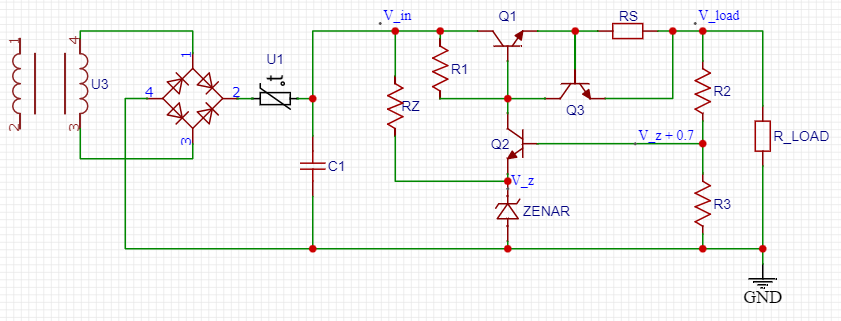
\includegraphics[height=1.9in]{Full circuit.png}\\
   \caption{Overall Circuit Diagram}
\end{figure}
\begin{multicols}{2}
\subsubsection{Regulation}
The final and maybe the most important task in a linear power supply is Regulation which ensures constant voltage. Regulation can be either shunt or series. A series regulator is connected in series with the load to stabilize the regulator's output voltage. A shunt regulator, on the other hand, is connected in parallel to the load to stabilize the device's output voltage. Since series regulators perform better in high currents than shunt regulators series regulation is used.\\
The regulation circuit consist of two sub circuits: Feedback circuit and over current protection circuit.
\subsubsection{Feedback Circuit}
Zener diode ensures the voltage across. Zener current should be controlled by the resistor Rz . For a proper operation of Zener the following conditions need to be satisfied,
$$I_K<I_Z<I_{max}$$
Resistors $R_2$ and $R_3$ act as potential dividers. Their resistance ratio ensures the output voltage.
\subsubsection{Over Current Protection Circuit} Transistor $Q_3$ act as over current protection and the biasing of it is controlled by the current sensing resistor $R_s$. $Q_3$ should forward biased when their is a current exceeding the rate in load.
$$V_{BE} = I_{Load}.R_s$$
Required $R_s$ value can be calculated from this equation.
\section{Method}
A $230/15 V$ transformer is used to step down the main ac power which is supposed to use according to the project description. There we get a peak voltage of $15\sqrt{2}V$ at the output end. This voltage is fed to the second phase, the rectifier. 
\begin{figure}[H]
   \centering
   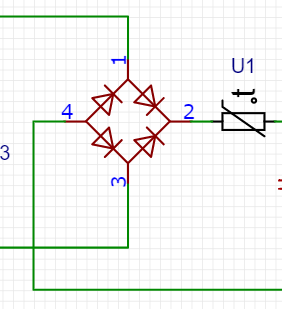
\includegraphics[height=1.7in]{rectification.png}\\
   \caption{Rectification}
\end{figure}
The PIV rating of the diodes in the rectifier bridge is as follows,\\
$$ PIV = V_p(sec) - 0.7V$$
$$=15\sqrt{2} - 0.7V$$
$$=20.5132V$$
From the rectifier we get an output of,\\
$$V_p(out) = V_p(sec) - 1.4V$$
$$ = 15\sqrt{2} - 0.7V$$
$$19.8132V$$
\begin{figure}[H]
   \centering
   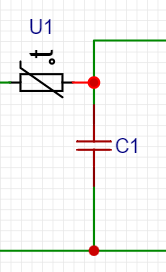
\includegraphics[height=1.7in]{Filtering.png}\\
   \caption{Filtering}
\end{figure}
Next, this voltage is fed to the filter.\\
At the filter, we should consider both the capacitance of the filter capacitor and the ripple of the output by the filter phase. We have come to a trade-off between ripple and the capacitor value.\\
The relationship between the ripple and the capacitance is achieved as follows,\\
$$V_{ripple} = \frac{I_{max}}{2.f.C}$$
$$I_{max}=10A,$$
$$V_{ripple} = \frac{10}{2 \times 100 \times C}$$
$$C=\frac{1}{20V_{ripple}}$$
For a capacitance of $ 4 \times 6800 $ $\mu $F (that is readily available in local markets) we get a ripple of around 1.8382V which is acceptable for our purpose.\\
Next, the smoothed DC wave is regulated by the series transistor regulator circuit. \\
After the smoothing, the DC voltage will drive a darlington transistor in the regulation circuit. The input current to the regulating circuit will divide into this darlington and a Zenar diode that is in the feedback circuit.
\begin{figure}[H]
   \centering
   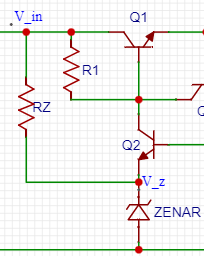
\includegraphics[height=1.8in]{Zenar.png}\\
   \caption{Regulation with Zenar Diode}
\end{figure}
Current that is going through the Zenar diode is a major consideration. It should be guaranteed that the diode is operating in it's reversed biased region.\\
$R_z$ value can control the current through the Zenar diode.\\
$$I_k < I_z < I_{max}$$
$$I_k < \frac{V_{in} - V_z}{R_z} < I_{max}$$
$$\frac{1}{I_k} > \frac{R_z}{V_{in}-V_z} > \frac{1}{I_{max}}$$
$$\frac{V_{in}-V_z}{I_k} > R_z > \frac{V_{in}-V_z}{I_{max}}$$
$$ R_z < \frac{(V_in - V_z)_{min}}{I_k} \&  R_z > \frac{(V_{in}-V_z)_{max}}{I_{max}}$$
$$\frac{19.8132 - V_z}{I_{max}} < R_z < \frac{(19.8132 - 1.8382) - V_z}{I_{Zk}}$$
\newline
1N4733A Zener diode is chosen and possible range of values for $R_z$ is calculated accordingly,\\
For 1N4733A zener diodes,\\
$I_{Zk} =1mA$, $I_{ZT} = 49mA$, $I_{Zm} = 179mA$ at $50$\textdegree $C.$
$$ \frac{(19.8132 - 5.1) V}{178mA} < R_z < \frac{(17.975-5.1)V}{1mA}$$
$$82.6584\Omega < R_z < 12875\Omega$$
\begin{figure}[H]
   \centering
   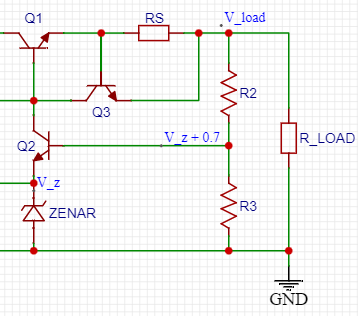
\includegraphics[height=1.8in]{Voltage Divider.png}\\
   \caption{Voltage Divider for Feedback}
\end{figure}
To ensure the 10V at the load end the $R_2$, $R_3$ resistors which are acting as potential divides in the feedback circuit ( base current to the $Q_2$ transistor is negligible), should maintain the proper ratio.\\
We get a Ratio between $R_2$ and $R_3$ as follows,\\
$$\frac{V_z + 0.7V}{R_3}(R_2+R_3) = 10V$$
$$\frac{R_2 + R_3}{R_3} =\frac{10}{5.1+0.7}$$
$$\frac{R_2}{R_3} = \frac{4.2}{5.8}$$
Practically it is hard to get the resistor ratio only by two resistors. Therefore a variable resistor is placed between two resistors to adjust the resistance ratio.
\subsection{Over-current Protection}
\begin{figure}[H]
   \centering
   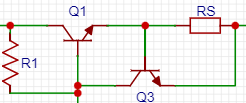
\includegraphics[height=1.3in]{Current Sensing.png}\\
   \caption{Over Current Protection}
\end{figure}
The $Q_3$ transistor will only be forward-biased whenever the current through the load exceeds 10A. So the current sensing resistor value should be,
$$R_4 = \frac{0.7}{10}$$
$$R_4 = 0.07\Omega$$
Whenever there is an over-current $Q_3$ will be forward biased and draw adequate collector current which ultimately results in a reduction of the base current of the Darlington Transistor $Q_1$. reduction in the base current of $Q_1$ will reduce the emitter current of $Q_1$ which is the main DC current to the load. Hence the load will be protected from over-currents.
\subsection{Heat Dissipation}
The MJ11016 NPN Darlington pair is used in the linear power supply design. Using the simulations in LTspice it is observed that, $73.5W$ amount of power is dissipated from the transistor package at the maximum required power output. This transistor dissipates higher amount of heat. Therefore, proper calculations should be done to determine whether the design need a heat sink and to determine the properties of the heat sink.\\
The maximum junction temperature rating for the MJ11016 Darlington transistor is mentioned as 200\textdegree C in the datasheet. For more safety, we can choose 80\% of that value which is 160\textdegree C.\\
\newline
Junction to Case thermal resistance for MJ11016 Darlington transistor, $R_{\theta JC}  = 0.87$\textdegree$C/W$\\  
\newline
Case to Sink thermal resistance for TO-3 package with mica, $R_{\theta CS}  = 0.36$\textdegree$C/W (Typical\: value)$\\
\newline
Sink to Ambient thermal resistance, $R_{\theta SA} = ?$ \\
\newline
$Maximum \: case \: temperature \\= 160$\textdegree $C - 0.87$\textdegree $C/W \times 73.5W = 96.055$\textdegree$C$\\
\newline
$Maximum \: heat sink \: temperature\\ = 96.055$\textdegree$C - 0.36$\textdegree $C/W \times 73.5W = 69.595$\textdegree$C$\\
\newline
$  R_{\theta SA}  =\frac{(69.595 - 28)\textdegree C} {73.5W }= 0.5659$\textdegree$C/W$\\
\newline
Therefore, the heat sink should have a thermal resistance less than  0.5659 \textdegree C/W.\\
In addition to the heat sink, a cooling fan is used to control the temperature inside the enclosure.
\subsection{Component Selection}
To select the components, LTspice was used as the simulation software to determine the power dissipated by each component and exact component values. According to those power requirements, transistors and resistors were selected.\\
Refer the \textcolor{blue}{\hyperlink{page.9}{component list}} generated using Altium Designer.

\section{Results}
The required output of 10V was perfectly achieved for no load condition accurate up to two decimal places. There is a small voltage drop 0f about 0.6V, when the load requires more current. \\
The maximum current that can be achieved from the power supply was 7.56A because the transformer is rated for 8A output.\\
Refer the \textcolor{blue}{\hyperlink{page.10}{data sheet}} to see the device specifications obtained from laboratory testings.
\subsection{PCB Design}
PCB design was done using Altium Designer. Track width and the PCB manufacturing material were major considerations during the design because this is a high power application.
\begin{figure}[H]
   \centering
   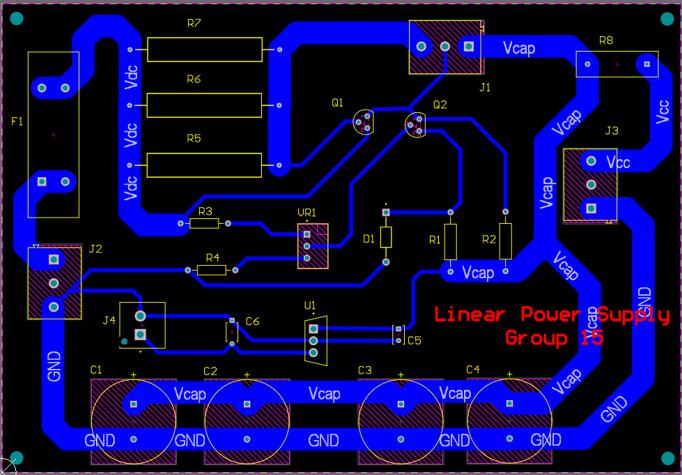
\includegraphics[ width=0.45\textwidth]{Results_PCB.png}\\
   \caption{PCB Design}
\end{figure}
\subsection{Enclosure Design}
Enclosure Design was done using Solidworks software. The linear power supply contains heating elements. Therefore, metal is chosen as the material to produce the enclosure for the linear power supply. The enclosure is designed as a block made from a metal sheet and during the assembly the sheet is folded to get the required appearance of the enclosure. Find additional images of the enclosure \textcolor{blue}{\hyperlink{page.12}{here}}.
\begin{figure}[H]
   \centering
   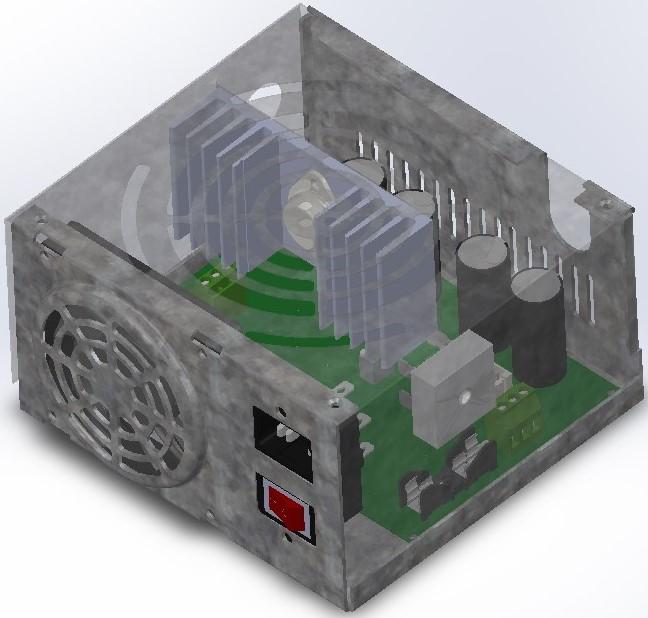
\includegraphics[ width=0.45\textwidth]{enclosure photos/img 1.jpg}\\
   \caption{Overall Enclosure Design}
\end{figure}

\section{Conclusion}
After studying the required specifications, every block of the circuit was analyzed, and the design met the required specifications (10V constant output) under low power conditions. But there is a slight voltage drop whenever the load requires high current, due to the inability of the transformer to produce 10A to the circuit. In this design, regulation is comparatively slow due to the use of a BJT as the feedback element instead of Op-amps.\\
Further, High power applications like this need proper safety methods to ensure the safety of the device and the user end. Proper grounding is essential for the device due to the metallic enclosure.\\
Aluminum is preferred over copper as the material for the PCB tracks due to the advantages in heat dissipation and thermal transfer than standard FR-4 constructions. \\


\section{Acknowledgement}
We would like to extend our deepest gratitude to
our supervisor Mr.Pramitha Muthukudarachchi, for his
valuable guidance, collaboration, patience, and
other essential instructions and comments provided
during progress meetings.
We must also thank all the academic lecturers, instructors,
and other academic staff whose contribution
indirectly helped us a lot in the completion
of this project successfully.
Finally, we would like to thank our fellow batch
mates for sharing their knowledge and experience
during the hard times.
\end{multicols}



\nocite{*}
\medskip
\bibliographystyle{ieeetr}
\bibliography{References}


\section{Contribution}
\begin{center}
\begin{tabular}{ |m{2.5cm}|m{4cm}|m{6cm}| } 
 \hline
 Index Number & Name & Contribution \\ 
 \hline
 190397E & Munasinghe B.S.V.W. & 
 \begin{itemize} 
            \item Circuit Design and Calculations 
            \item Testing Simulations 
            \item Component Selection 
            \item Soldering and Final Assembly
        \end{itemize}  \\ 
 \hline
 190399L & Munasinghe M.M.R.H. &
 \begin{itemize} 
            \item Circuit Design and Calculations
            \item PCB Design
            \item Component Selection 
        \end{itemize}  \\ 
 \hline
 190413D & Nifla M.N.F. &
 \begin{itemize} 
            \item Circuit Design and Calculations
            \item Simulation Schematic Design 
            \item Documentation 
        \end{itemize}  \\ 
 \hline
 190423H & Nushath M.N.M. &
 \begin{itemize} 
            \item Simulation Schematic Design
            \item Enclosure Design 
            \item Component Selection  
        \end{itemize}  \\ 
 \hline
\end{tabular}
\end{center}


\section{Appendices}


\subsection{Appendix I - PCB Schematic}
Click \textcolor{blue}{\hyperlink{page.8}{here}}
\begin{figure}
    \centering
    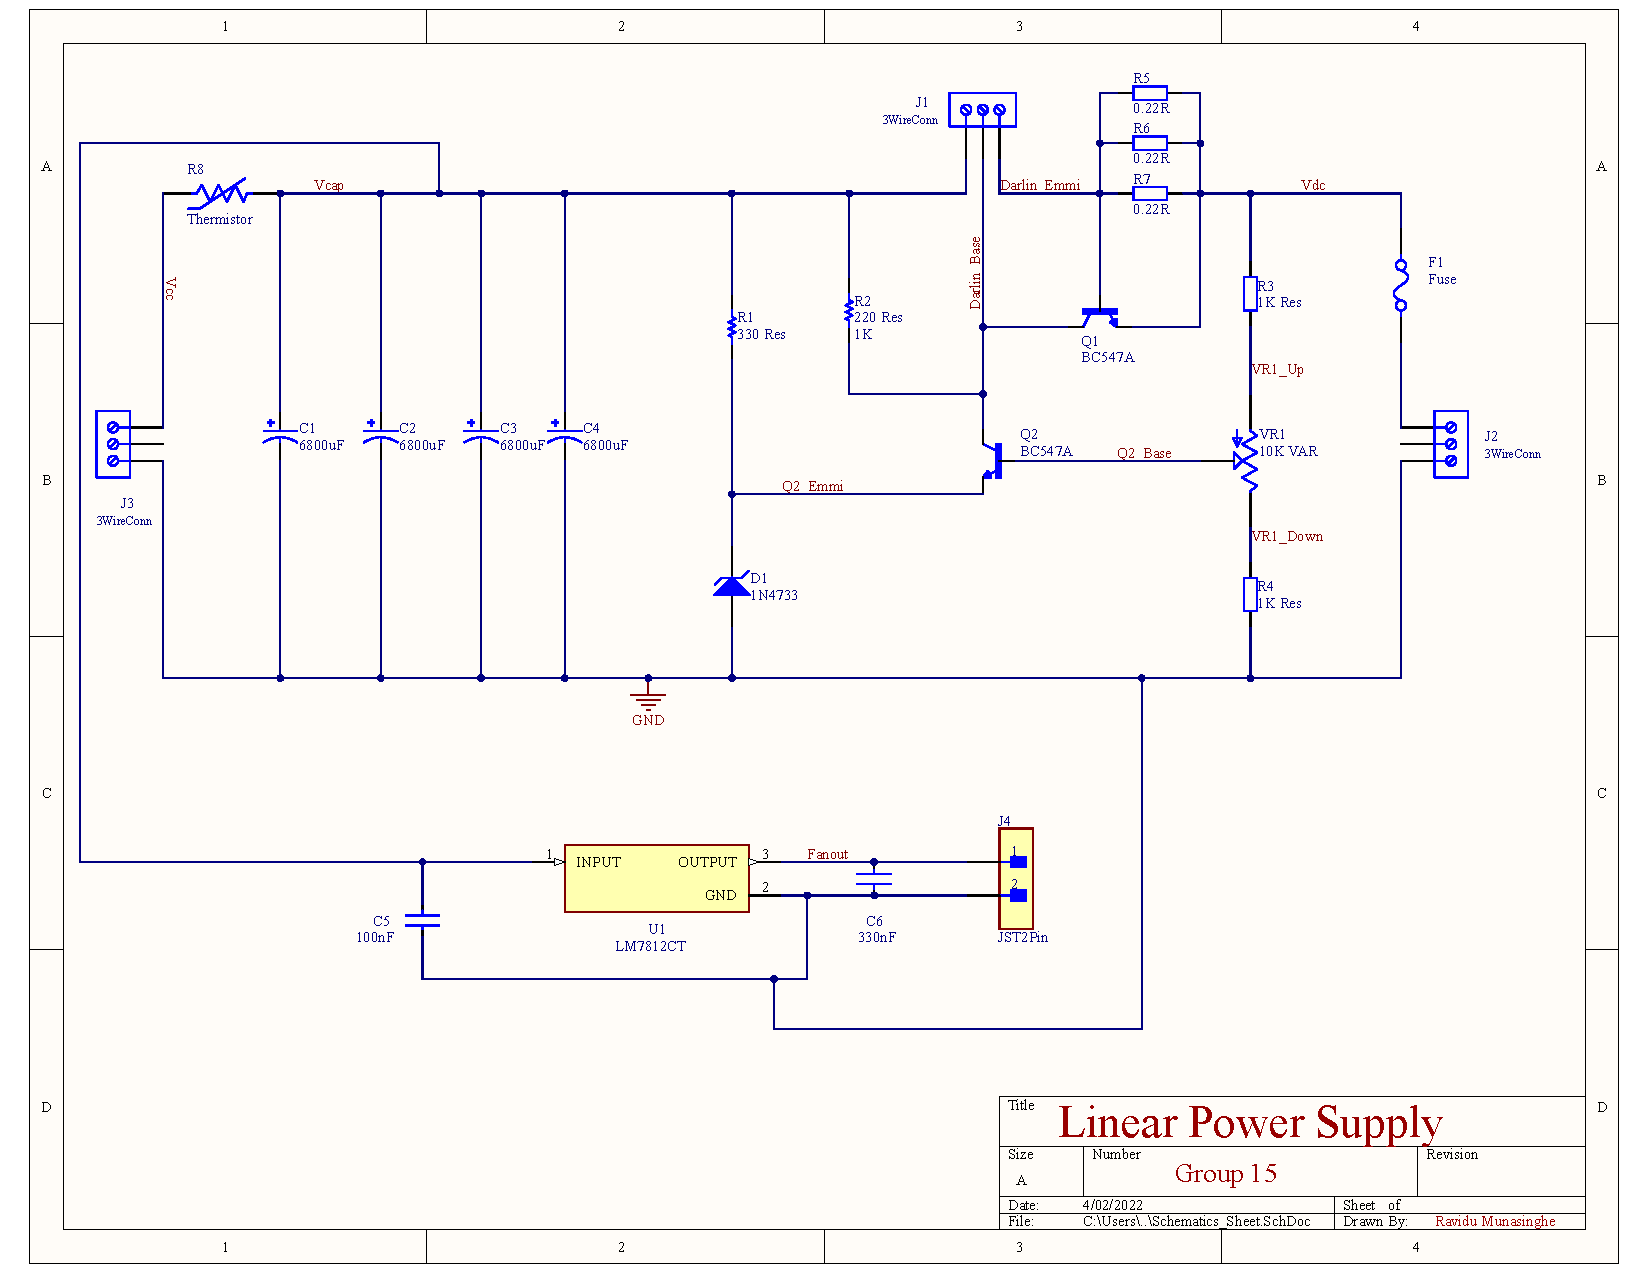
\includegraphics[width=1\textwidth]{schematic.pdf}
\end{figure}

\subsection{Appendix II - Component List}
Click \textcolor{blue}{\hyperlink{page.9}{here}}
\label{sec:components}
\begin{figure}
    \centering
    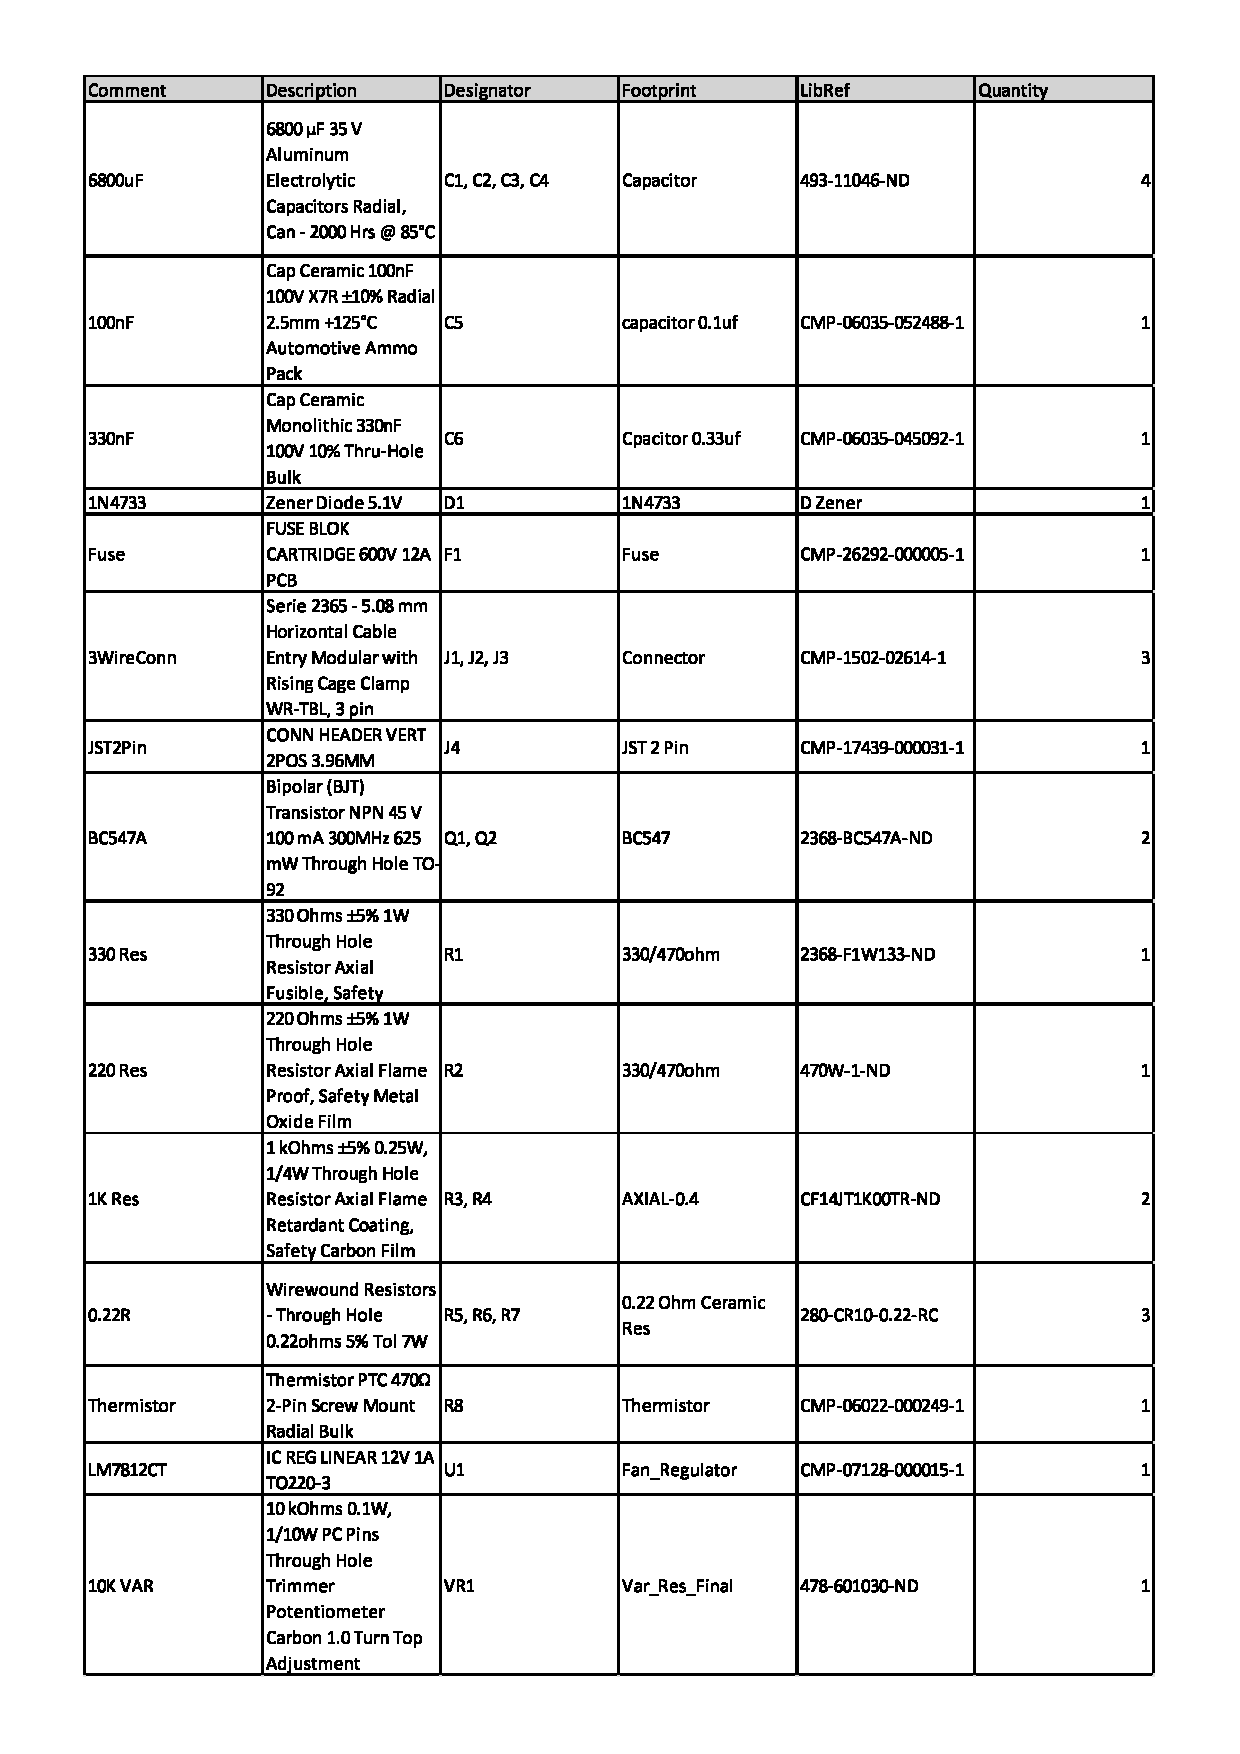
\includegraphics[width=0.9\textwidth]{qq2.pdf}
\end{figure}

\subsection{Appendix III - Data sheet}
Click \textcolor{blue}{\hyperlink{page.10}{here}}
\begin{figure}
    \centering
    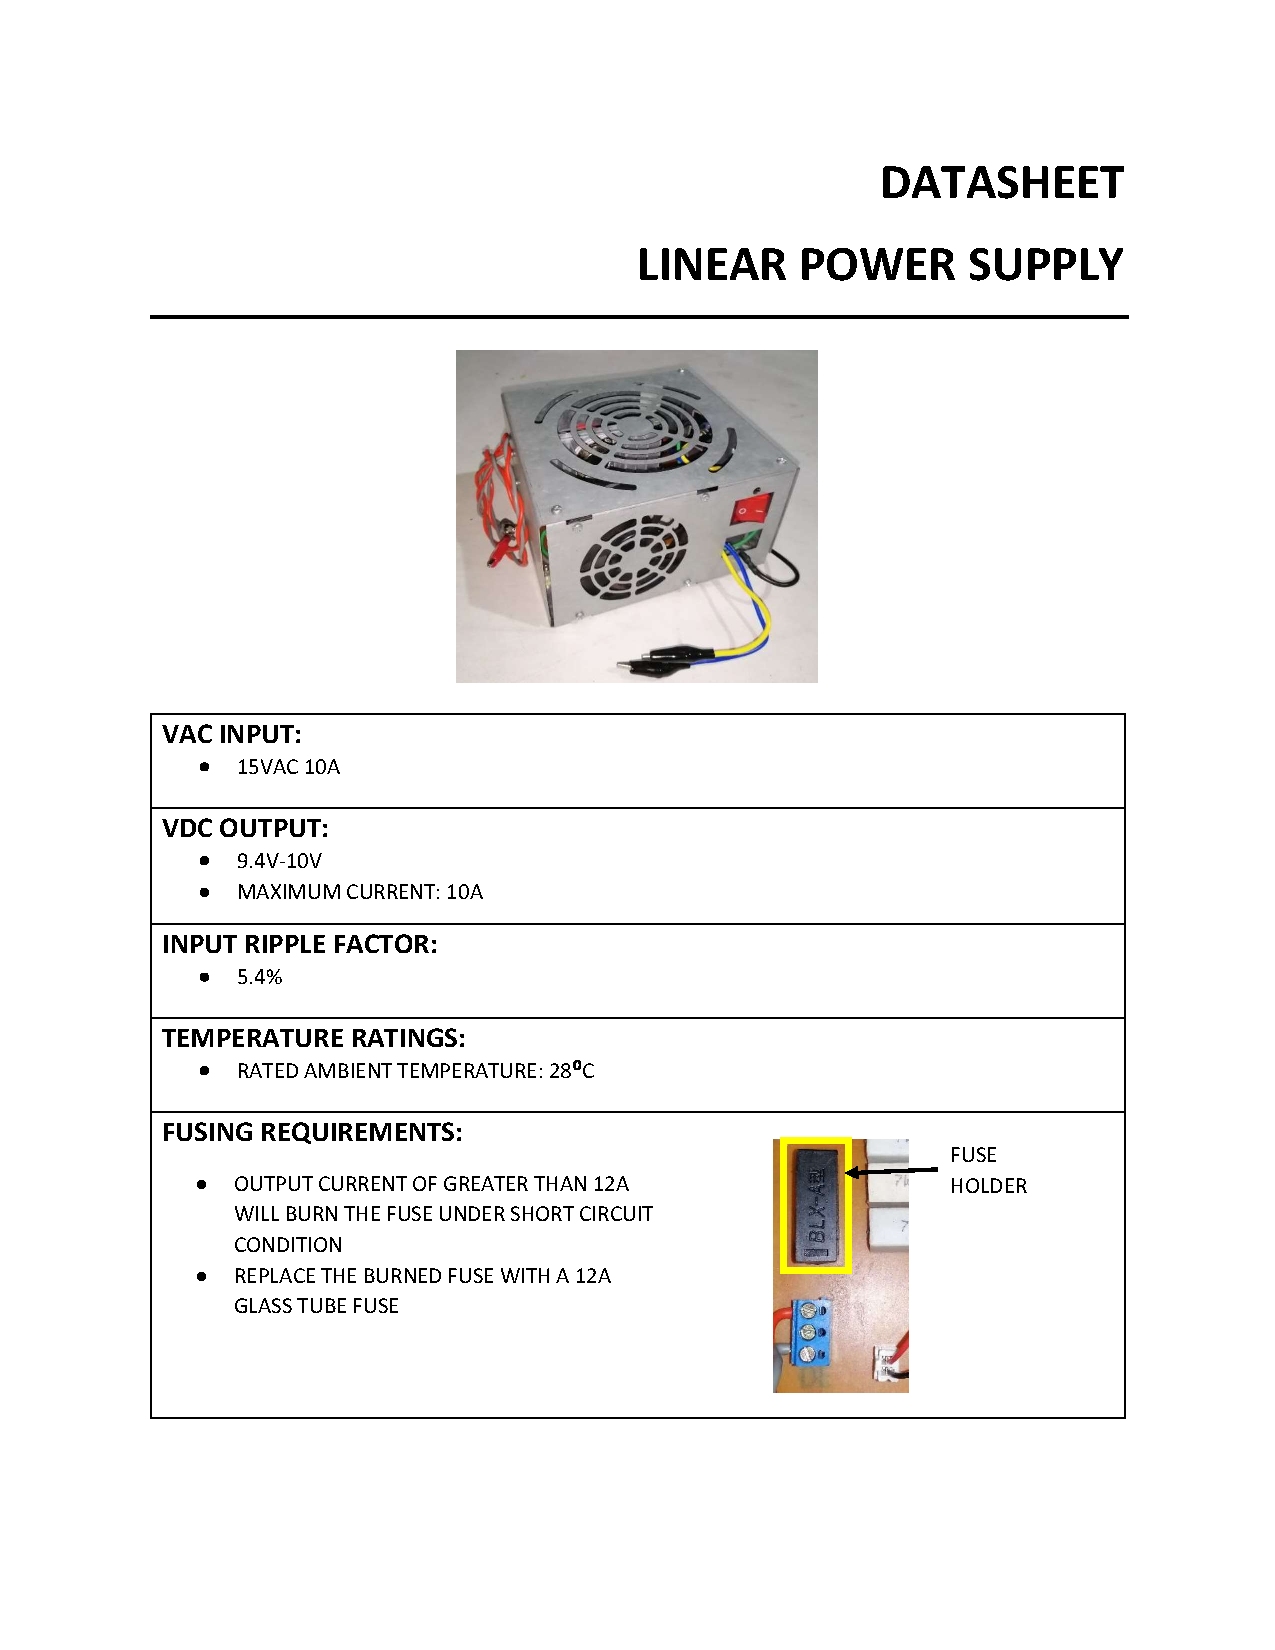
\includegraphics[width=1\textwidth]{DS1.pdf}
\end{figure}

\begin{figure}
    \centering
    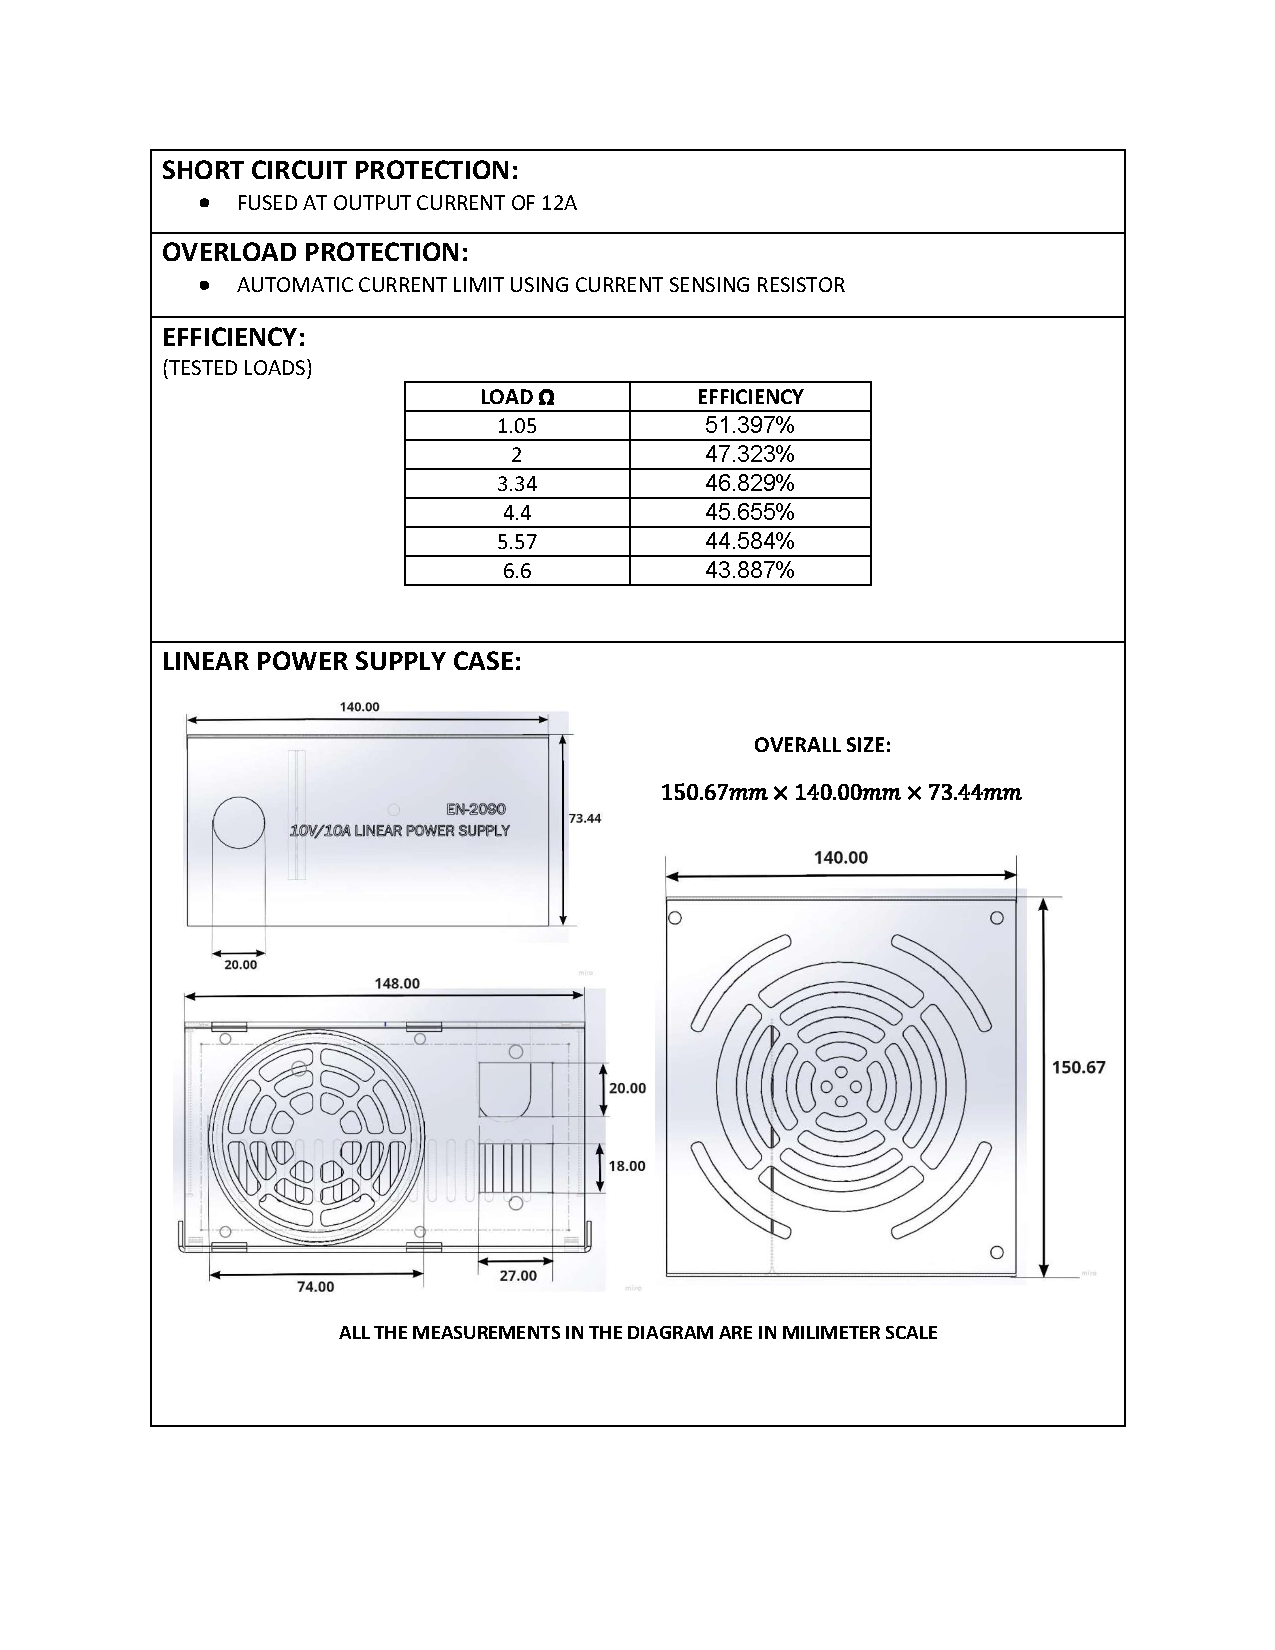
\includegraphics[width=1\textwidth]{DS2.pdf}
\end{figure}


\subsection{Appendix IV - Enclosure}
Click \textcolor{blue}{\hyperlink{page.12}{here}}
\label{sec:enc}
\begin{multicols}{2}
\begin{figure}[H]
    \centering
    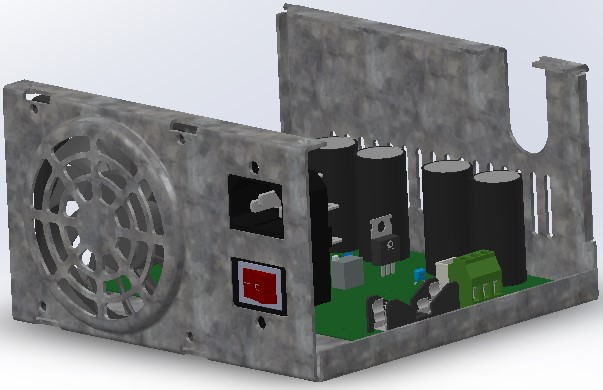
\includegraphics[width=0.5\textwidth]{enclosure photos/sss1.jpg}
    \caption{Enclosure Part I Front}
\end{figure}

\begin{figure}[H]
    \centering
    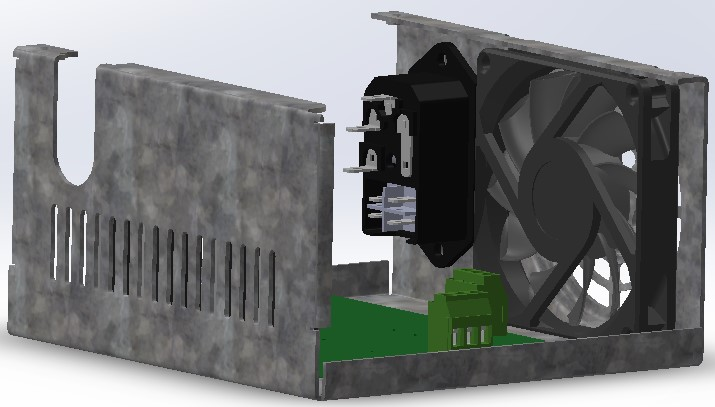
\includegraphics[width=0.5\textwidth]{enclosure photos/sss2.jpg}
    \caption{Enclosure Part I Back}
\end{figure}
\end{multicols}

\begin{multicols}{2}
\begin{figure}[H]
    \centering
    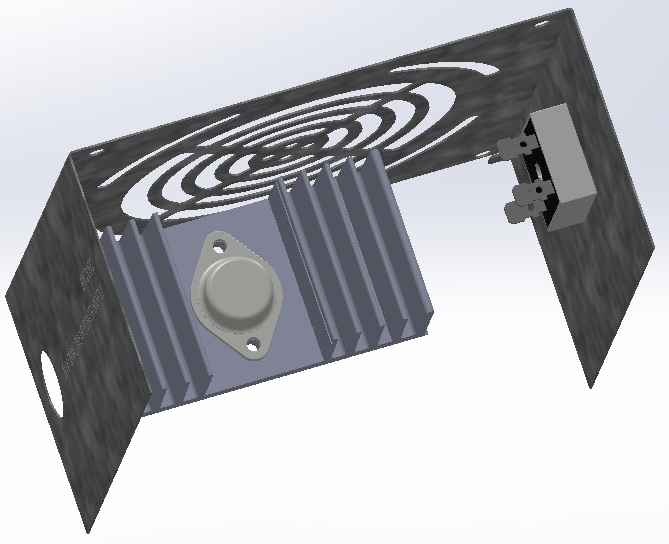
\includegraphics[width=0.5\textwidth]{enclosure photos/img 4.jpg}
    \caption{Enclosure Part II Front}
\end{figure}

\begin{figure}[H]
    \centering
    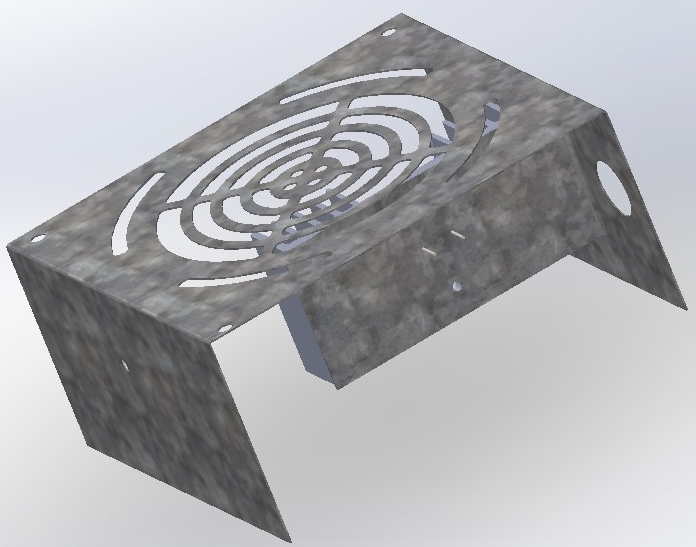
\includegraphics[width=0.5\textwidth]{enclosure photos/img 5.jpg}
    \caption{Enclosure Part II Back}
\end{figure}
\end{multicols}


\begin{figure}[H]
    \centering
    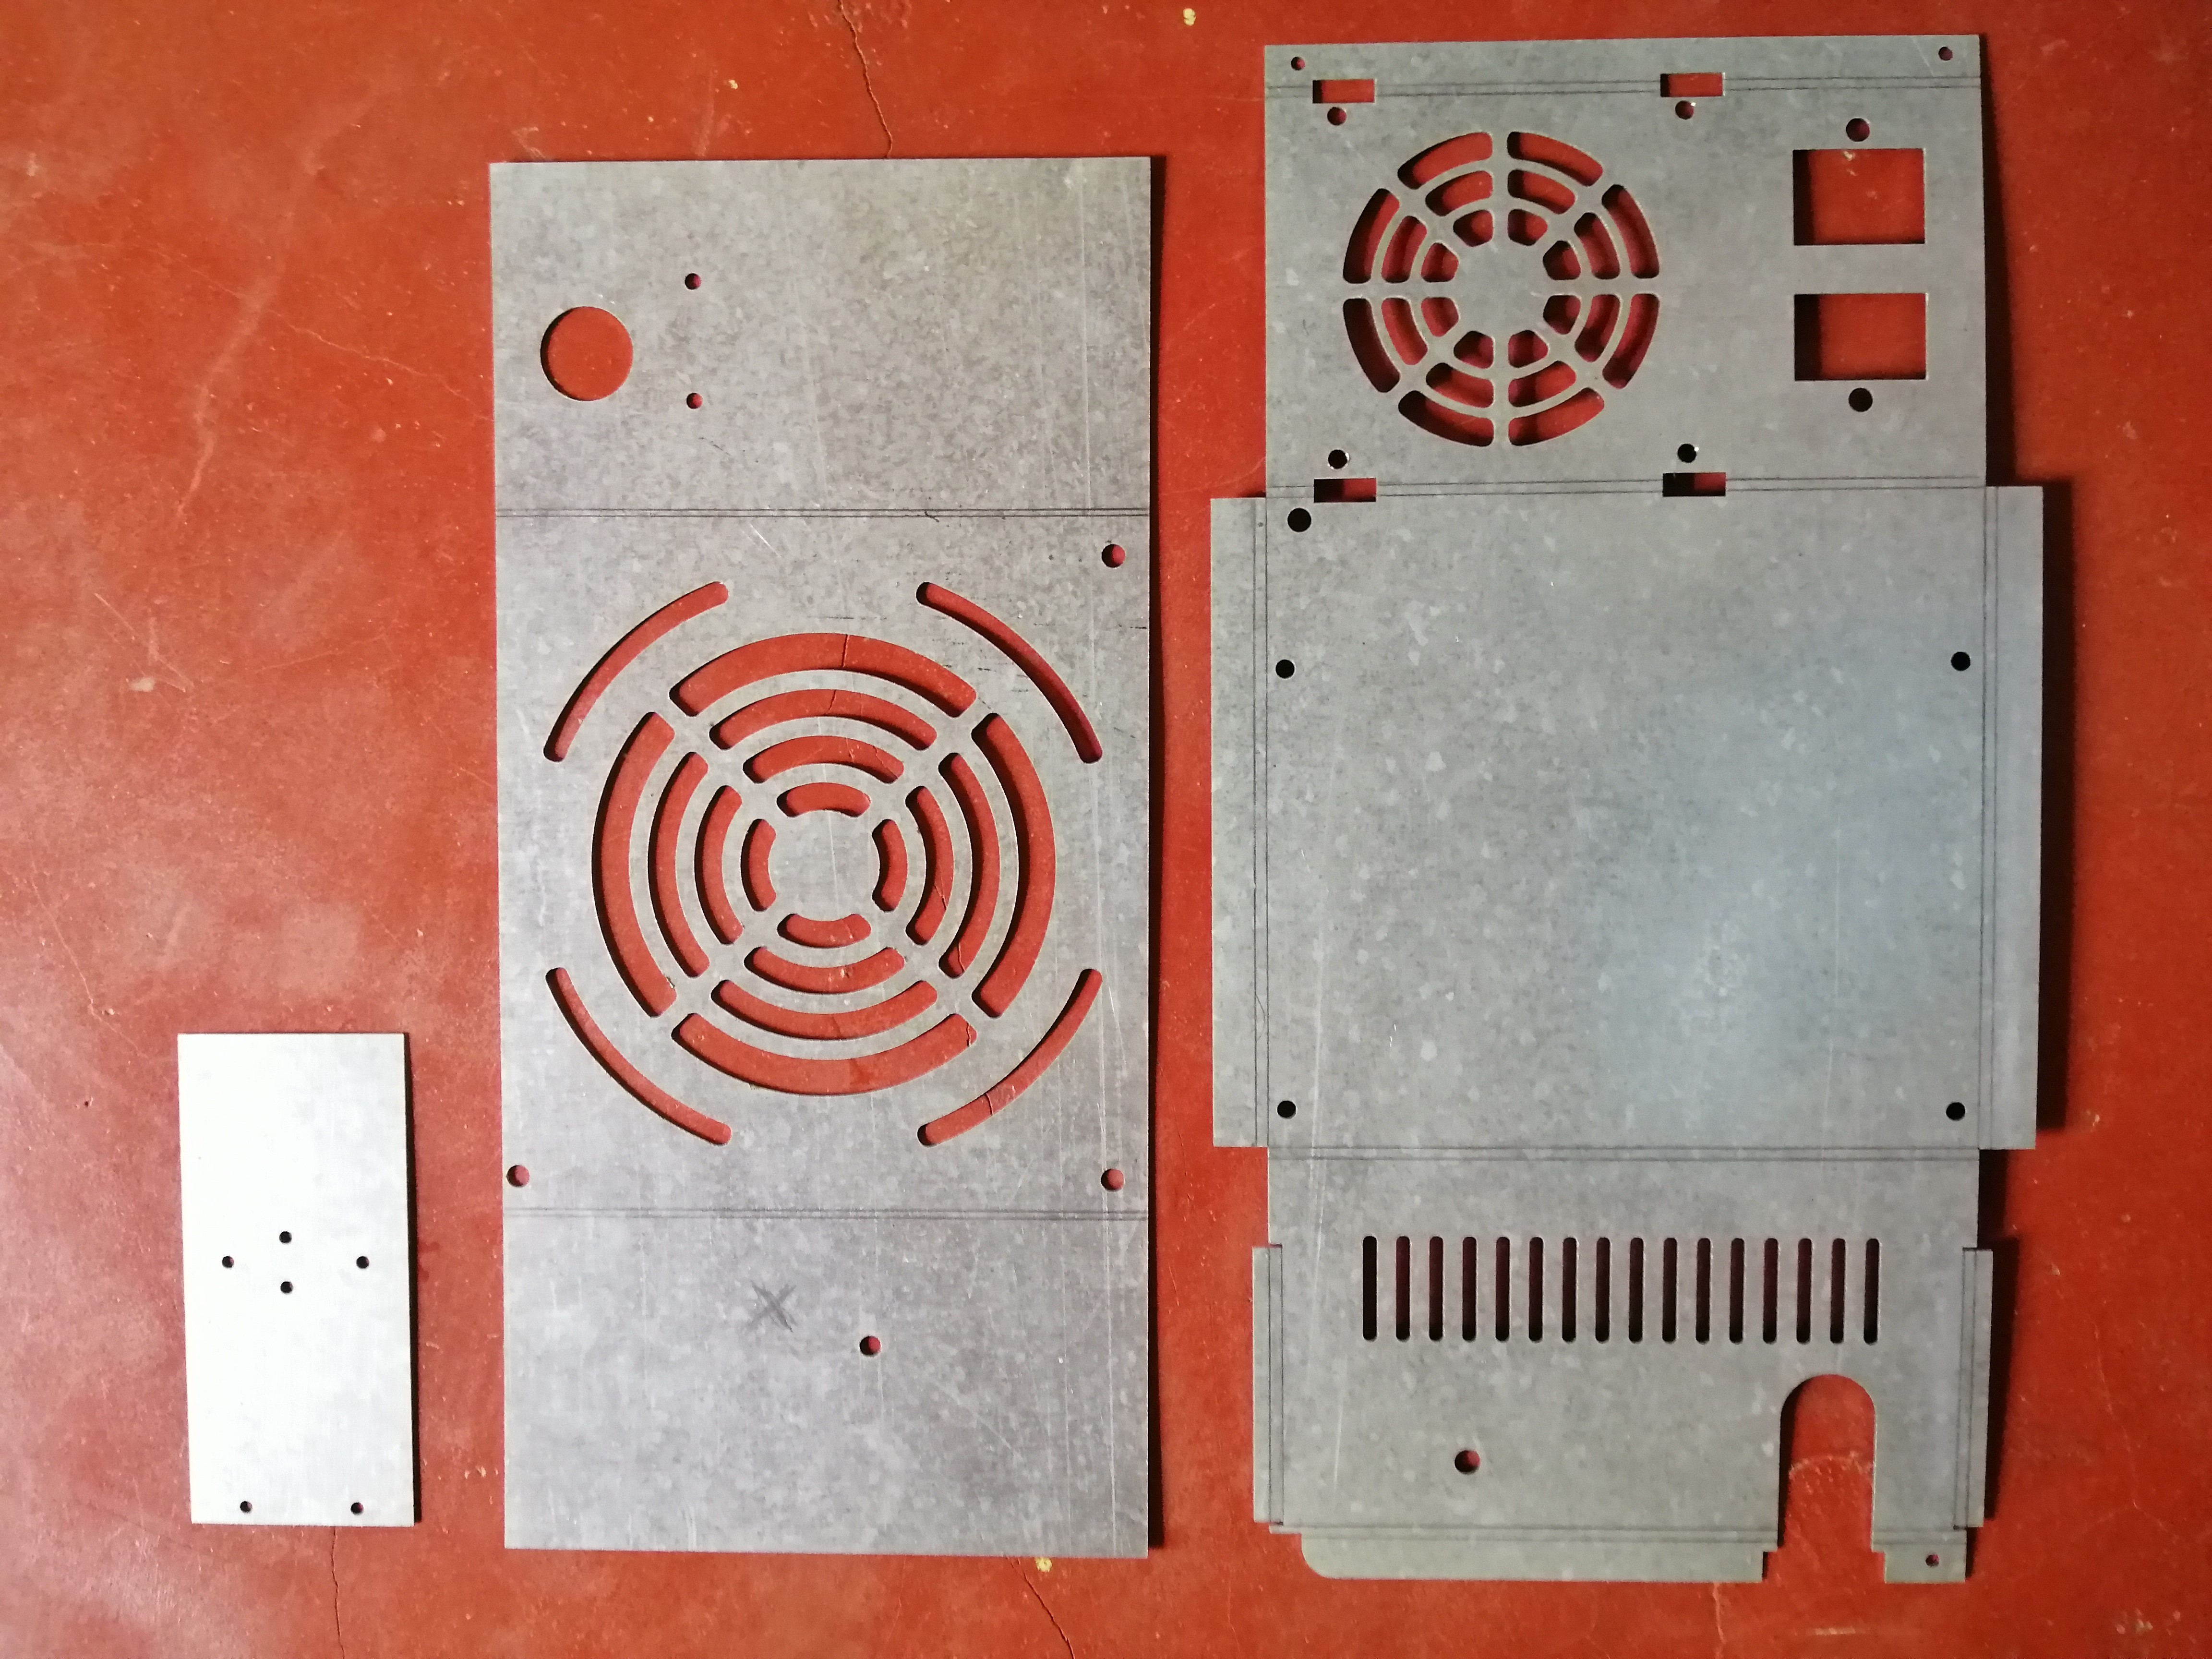
\includegraphics[width=0.7\textwidth]{block_enclosure.jpg}
    \caption{Enclosure Block}
\end{figure}

\begin{figure}[H]
    \centering
    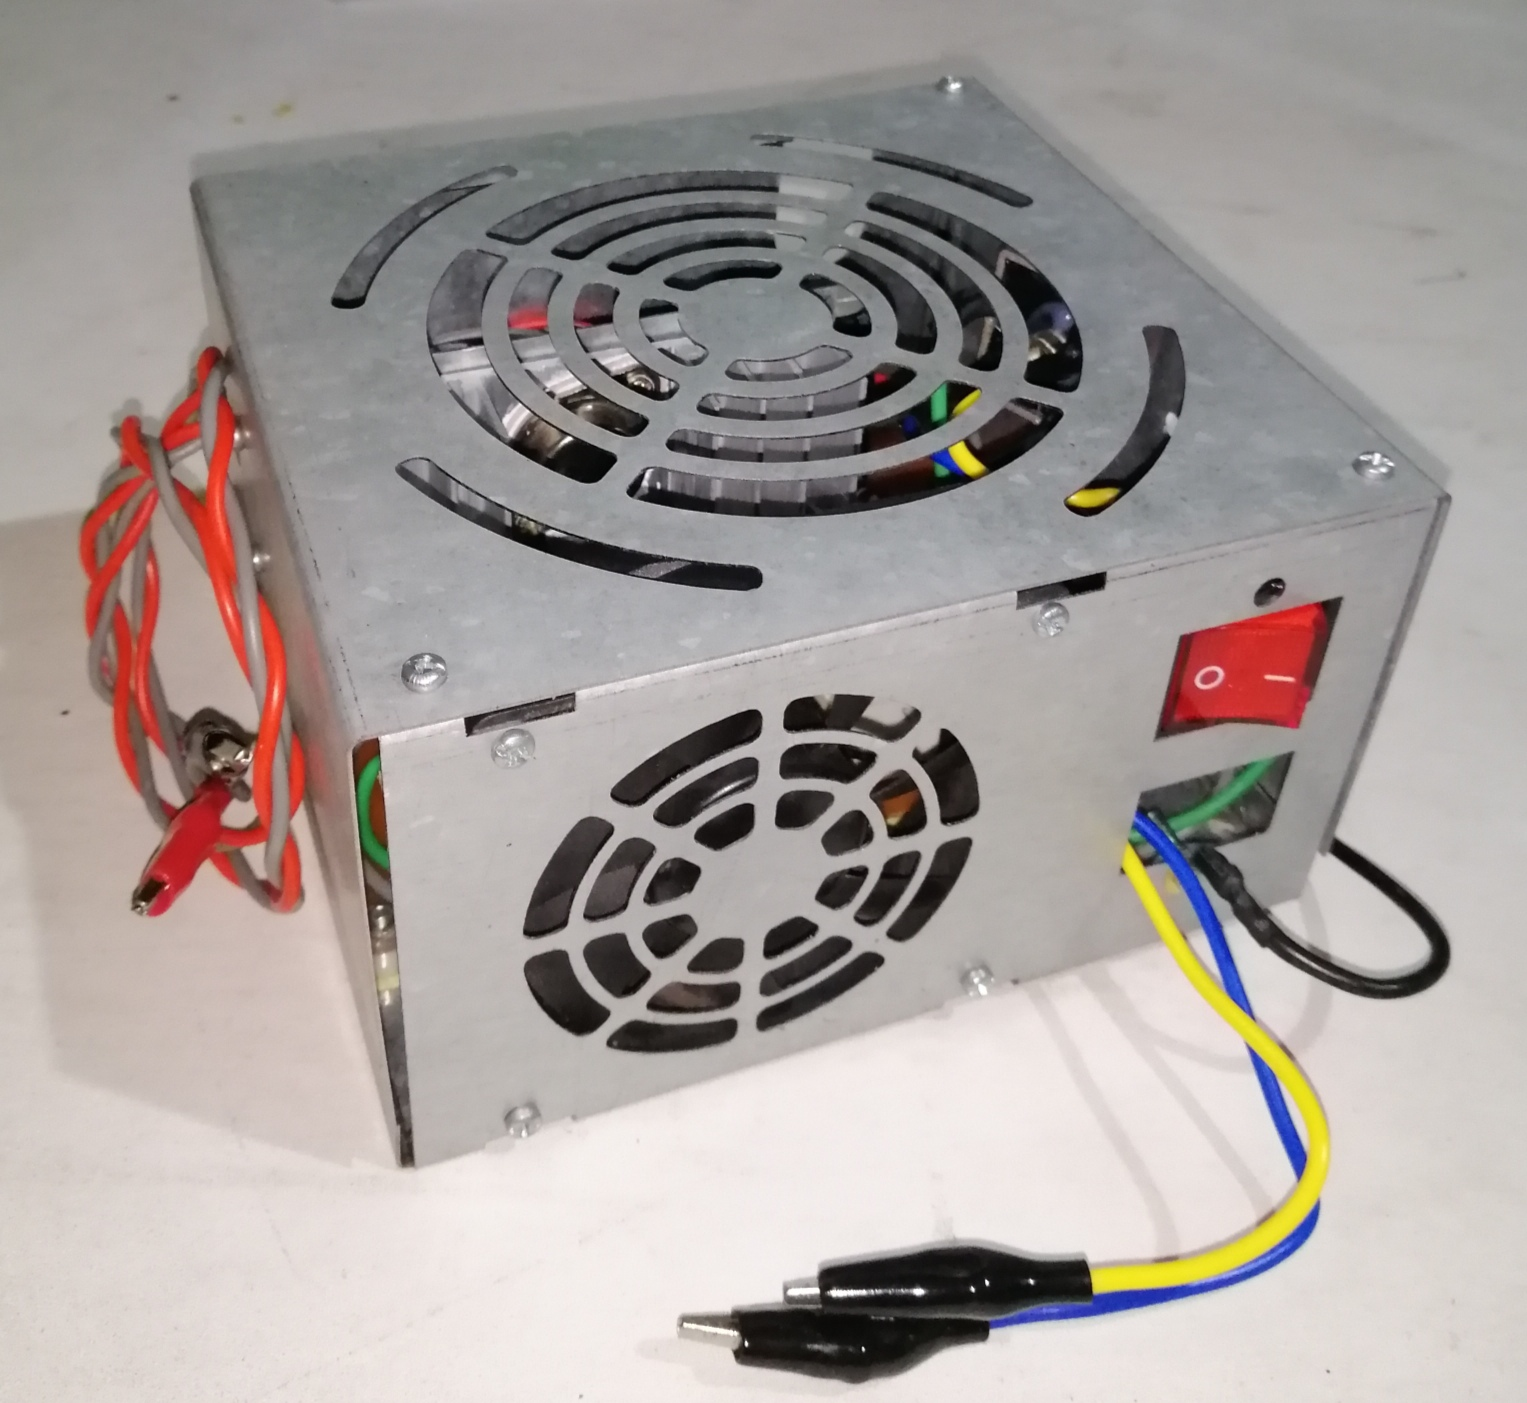
\includegraphics[width=0.7\textwidth]{LPS.jpg}
    \caption{Assembled Product}
\end{figure}




\end{document}